%%%%%%%%%%%%%%%%%%%%%%%%%%%%%%%%%%%%%%%%%%%%%%%%%%%%%%%%%%%%%%%%%%%%%%%%%%%%%%%%
%2345678901234567890123456789012345678901234567890123456789012345678901234567890
%        1         2         3         4         5         6         7         8

%\documentclass[letterpaper, 10 pt, conference]{ieeeconf}  % Comment this line out if you need a4paper

\documentclass[a4paper, 11pt, conference]{ieeeconf}      % Use this line for a4 paper

\IEEEoverridecommandlockouts                              % This command is only needed if 
                                                          % you want to use the \thanks command

% \overrideIEEEmargins                                      % Needed to meet printer requirements.

%In case you encounter the following error:
%Error 1010 The PDF file may be corrupt (unable to open PDF file) OR
%Error 1000 An error occurred while parsing a contents stream. Unable to analyze the PDF file.
%This is a known problem with pdfLaTeX conversion filter. The file cannot be opened with acrobat reader
%Please use one of the alternatives below to circumvent this error by uncommenting one or the other
%\pdfobjcompresslevel=0
%\pdfminorversion=4

% See the \addtolength command later in the file to balance the column lengths
% on the last page of the document

% The following packages can be found on http:\\www.ctan.org
%\usepackage{graphics} % for pdf, bitmapped graphics files
%\usepackage{epsfig} % for postscript graphics files
%\usepackage{mathptmx} % assumes new font selection scheme installed
%\usepackage{times} % assumes new font selection scheme installed
%\usepackage{amsmath} % assumes amsmath package installed
%\usepackage{amssymb}  % assumes amsmath package installed
\usepackage[english]{babel}
% Set page size and margins
% Replace `letterpaper' with `a4paper' for UK/EU standard size
\usepackage[letterpaper,top=2cm,bottom=2cm,left=3cm,right=3cm,marginparwidth=1.75cm]{geometry}
% Useful packages
\usepackage{amsmath}
\usepackage{graphicx}
\graphicspath{ {./images/} }
\usepackage[colorlinks=true, allcolors=blue]{hyperref}
\usepackage{float}
\usepackage{subcaption}
\usepackage{algorithmicx}
\usepackage{algpseudocode}
\usepackage[
backend=biber,
style=numeric,
sorting=none
]{biblatex}
\addbibresource{references.bib}

\title{\LARGE \bf Multi-Agent Planning to Detect Obstacles and Navigate in an Unknown Environment}


\author{
  Agarwal, Shantnav\\
  \text{5939933}
  \and
  Deshmukh, Shlok\\
  \text{5928516}
  \and
  Singh, Manupriya\\
  \text{6050425}
  \and
  Theocharous, Alexandros\\
  \text{5930901}
}


\begin{document}



\maketitle
\thispagestyle{empty}
\pagestyle{empty}


%%%%%%%%%%%%%%%%%%%%%%%%%%%%%%%%%%%%%%%%%%%%%%%%%%%%%%%%%%%%%%%%%%%%%%%%%%%%%%%%
\begin{abstract}
 Rescue operations for individuals lost in a forest can use drones to quickly scan a large unknown environment and provide relief. We propose a solution by making multiple drones cooperatively scan the entire area. Through a simulation we show that the combination of an efficient global and local planner can reduce search time significantly.
\end{abstract}

%%%%%%%%%%%%%%%%%%%%%%%%%%%%%%%%%%%%%%%%%%%%%%%%%%%%%%%%%%%%%%%%%%%%%%%%%%%%%%%%
\section{INTRODUCTION}
Objective:
\begin{enumerate}
    \item Multiple drones plan and scan the unknown environment. The unknown environment is broken down into multiple grids and the task of the drones is to visit each grid in a cooperative manner.
    \item The drones detect obstacles around them which are then transformed to the initial frame and updated on a common map.
    \item When a person is found, a different drone using the common map calculates the optimal path to reach their location and provide relief.
\end{enumerate}
Environment:
\begin{enumerate}
    \item We will use PyBulletDrone environment for this project where cylinders are used to represent trees.
    \item The environment spawns these trees at random locations throughout the map which is unknown to the planning algorithm. These obstacles are sensed by the robot as they come within the sensing range of onboard sensors.
    \item A person is said to be detected when the drone is close enough to their location.
\end{enumerate}
Procedure:
\begin{enumerate}
    \item Our workspace is \(R^3\). Configuration space of the quadcopter is \(R^3 \times SO(3)\). We will plan in the workspace \(R^3\) itself. \textcolor{red}{Should we search for the optimal path in the 3D World space or the 6D C-Space of the robot or 12D Position + Velocity space? We can use kinodynamics of the quadrotor to simplify the problem.}
    \item We use a high level planner that directs the drones to scan the environment in a Breadh first search manner. The robots communicate with a central node that directs the search such that 2 drones do not explore the same region.
    \item The drone gets its next target location from the high level planner. We use the \(RRT^*\) algorithm on the common map to plan the path for the drone from its current location to the target location.
    \item We use the \(RRT^*\) algorithm over \(A^*\) because the entire map is not known. As \(RRT^*\) builds the tree incrementally, we can update the path with new information without recomputing the map entirely.
    \item Then make the quadcopters follow this path using an off the shelf control algorithm.
    \item The algorithm will be evaluated on the time taken to find the lost person and the the time taken to provide aid to the person once found.
\end{enumerate}

\section{ROBOT MODEL}
% 1/2-1 page
 
We have decided to use Quadrotor as our robot. Quadrotor's workspace and configuration space are \(R^3\) and  \(R^3 \times SO(3)\), respectively.
The derivation of the dynamics is as follows\cite{6289431}.
\subsection{Model of a rotor}

Each rotor rotates with angular velocity $\omega$ and generates a lift force F and moment M. Moment is acting opposite to the directing of rotation.

The lift Force F and moment M of ith rotor can be calculated by:

$F_i = k_f * \omega_i^2$, \hspace{1cm} $k_f = k_T*\rho * D^4$

$M_i = k_m * \omega_i^2$, \hspace{1cm} $k_m = k_Q*\rho * D^5$

where:

%$k_T$ is thrust coefficient

%$k_Q$ is torque 

%$rho$ is fluid density

%$D$ is diameter of propeller

\subsection{Equations of Motion}

Total thrust and moment is the sum of individual ones in each of the 4 rotors.

Thrust: $F = \sum F_i - mga_3$

%Here, $F_x$ are individual lift forces by the propellers and $m*g$ is the one by gravity.

Moment: $M = \sum r_i*F_i + \sum M_i$

%Here, $r_i*F_i$ are the moments created by forces in quadrotor's centre of gravity and $M_x$ are the individual moments created by the propellers.


\subsection{Newton-Euler Equations for Quadrotor}

\textit{Linear Dynamics}:

Applying Newton's Second Law for system of particles, we get (in inertial frame);

$F = m * a$ 

%$acceleration (\ddot{r}) = d\dot{r}/dt$, where $\dot{r} = [u,v,w]^T$ (3.3)
In matrix form, we get;

\[
m*\ddot{r} = \begin{bmatrix}
    0 \\
    0 \\
    -m*g
\end{bmatrix} + 
R_\psi\phi\theta \begin{bmatrix}
    0 \\
    0 \\
    \sum F_i
\end{bmatrix}
\]
\\

\textit{Rotational Dynamics}:

%Applying Euler's rotation equations, we get (in body frame);

%$M_c = ^AdH_c^B/dt = ^BdH_c^B/dt + ^A\omega^B \times H_c^B$

%where, $H_c$ is the angular momentum and $^A\omega^B$ is angular velocity of body B in frame A which is given by $p.b_1 + q.b_2 + r.b_3$

Applying General vector form of Euler's equation;
$M_c = I\dot{\omega} + \omega \times (I\omega)$

For Quadrotor, after rearranging the general vector form, we get;
\[
I\begin{bmatrix}
    \dot{p} \\
    \dot{q} \\
    \dot{r}
\end{bmatrix} = 
\begin{bmatrix}
    L(F_2 - F_4) \\
    L(F_3 - F_1) \\
    M_1 - M_2 + M_3 - M_4
\end{bmatrix} - 
\begin{bmatrix}
    p \\
    q \\
    r
\end{bmatrix}
\times I\begin{bmatrix}
    p \\
    q \\
    r
\end{bmatrix}
\]

Let $\gamma = k_M/k_F$, $M_i = \gamma F_i$, we get;

\[
I\begin{bmatrix}
    \dot{p} \\
    \dot{q} \\
    \dot{r}
\end{bmatrix} = 
\begin{bmatrix}
    0 & L & 0 & -L \\
    -L & 0 & L & 0 \\
    \gamma & -\gamma & \gamma & -\gamma
\end{bmatrix}
\begin{bmatrix}
    F_1 \\
    F_2 \\
    F_3 \\
    F_4
\end{bmatrix}- 
\begin{bmatrix}
    p \\
    q \\
    r
\end{bmatrix}
\times I\begin{bmatrix}
    p \\
    q \\
    r
\end{bmatrix}
\]

Final equations using Linear and Rotational dynamics equations, we get;

\[
\begin{bmatrix}
    T \\
    \tau_1 \\
    \tau_2 \\
    \tau_3
\end{bmatrix} = 
\begin{bmatrix}
    k_F & k_F & k_F & k_F \\
    0 & Lk_F & 0 & -Lk_F \\
    -Lk_F & 0 & Lk_F & 0 \\
    k_M & -k_M & k_M & -k_M
\end{bmatrix}
\begin{bmatrix}
    \omega_1^2 \\
    \omega_2^2 \\
    \omega_3^2 \\
    \omega_4^2
\end{bmatrix}
\]

%TODO shorten, narrative, separate in paragraphs

%\subsection{State Variables}

%$u, \phi, p$ are the linear velocity along the roll-axis direction, angle rotated and the angular velocity about the roll-axis.
%$w, \psi, r$ is the linear velocity along the yaw-axis direction, angle rotated and the angular velocity about the yaw-axis.
%$v, \theta, q$ is the linear velocity along the pitch-axis direction, angle rotated and the angular velocity about the pitch-axis.
%$x, y, z$ are the position of quadrotor along $a_1, a_2, a_3$ axis of the inertial frame. 

%\begin{figure}[H]
%    \centering
%    \includegraphics[width=0.5\linewidth]{variables.png}
%    \caption{Inertial frame a and body frame b}
%    \label{fig:enter-label}
%\end{figure}


%\subsection{Rotation Matrices}

%We have five coordinate reference frames in total. Namely, Inertial frame, vehicle frame, yaw-adjusted frame, pitch adjusted frame and body frame. Inertial frame is fixed on the ground at a predefined home location ($a_1, a_2, a_3$).Vehicle frame has axes parallel to the inertial frame but has the origin shifted to the quadrotor’s center of gravity. Vehicle frame’s yaw is adjusted to match the quadrotor’s yaw to get the yaw-adjusted frame which is then pitch adjusted to get pitch-adjusted frame. Finally body frame is obtained by adjusting the roll of the pitch adjusted frame. The transformation from the inertial to vehicle frame is just as simple translation. The transformation from vehicle to body frame ($b_1, b_2, b_3$) is given by the following rotation matrix:
%\vspace{10pt}

%$R_v^b(\phi, \theta, \psi) = R_p^b(\phi)R_y^p(\theta)R_v^y(\psi)$

%\[
%= \begin{bmatrix}
%    1 & 0 & 0 \\
%    0 & $cos\phi$ & $sin\phi$ \\
%    0 & $-sin\phi$ & $cos\phi$ \\
%\end{bmatrix}.
%\begin{bmatrix}
%    $cos\theta$ & 0 & $-sin\theta$ \\
%    0 & 1 & 0 \\
%    $sin\theta$ & 0 & $cos\theta$
%\end{bmatrix}
%\begin{bmatrix}
    
%\]

%\subsection{Kinematics}

%\subsubsection{Translational Kinematics}
%The state variables(\(\dot{x}\), \(\dot{y}\), \(\dot{z}\)) are inertial frame parameters whereas, velocities ($u, v, w$) are body frame parameters. They can be related through the transformation matrix as follows:

%\[
%\begin{bmatrix}
%  \dot{x} \\
%  \dot{y} \\
%  \dot{z}
%\end{bmatrix} = 
%(R_v^b)^T \cdot \begin{bmatrix}
%    $u$ \\
%    $v$ \\
%    $w$     
%\end{bmatrix}
%\]

%\subsubsection{Rotational Kinematics}
%Since the yaw(relative to vehicle frame), pitch(relative to yaw-adjusted frame) and roll(relative to pitch-adjusted frame) are measured relative to different coordinate systems, the transformation for each is different. So, the angular velocities (p,q,r) are obtained as follows:

%\[
%\begin{bmatrix}
%  p \\
%  q \\
% r
%\end{bmatrix} = 
%\begin{bmatrix}
%    \dot{\phi} \\
%    0 \\
%    0     
%\end{bmatrix} + 
%R_p^b(\phi) \cdot \begin{bmatrix}
%    0 \\
%    \dot{\theta} \\
%    0     
%\end{bmatrix} +
%R_p^b(\phi) \cdot R_y^p(\theta) \cdot \begin{bmatrix}
%    0 \\
%    0 \\
%    \dot{\psi}     
%\end{bmatrix}
%= \begin{bmatrix}
%    1 & 0 & -sin\theta \\
%    0 & cos\theta & sin\phi cos\theta \\
%    0 & -sin\phi & cos\phi cos\theta
%\end{bmatrix} 
%\cdot \begin{bmatrix}
%    \dot{\phi} \\
%    \dot{\theta} \\
%    \dot{\psi}
%\end{bmatrix}
%\]

\section{MOTION PLANNING}
% 1/2-1 page
%! Date = 08/01/24

\subsection{Global Path Planning}

For global path planning, the environment is represented as a grid of a certain area size. The objective is to provide separate paths for all the drones while covering all the cells in the grid. A breadth-first search (BFS) strategy is employed for our multi-drone global path planning algorithm. BFS is chosen for its completeness. In BFS, one vertex is selected at a time, visited, and marked, and then its adjacent vertices are visited and stored in the queue. This process ensures that all cells are covered.

\subsubsection{GlobalPlanner Class}

\begin{itemize}
    \item \textit{\_\_init\_\_(self, drone\_id, start):} Initialize a drone with a unique ID and starting position.
    \item \textit{move(self, grid, queue, visited):} Attempts to move the drone to neighboring cells based on a 2D grid. If a valid move is found, the drone updates its position, marks the new cell as visited, and appends the position to its path.
\end{itemize}

\subsubsection{bfs\_multi\_drones Function}

\begin{itemize}
    \item Accepts the size of the grid (\textit{grid\_size}) and the number of drones (\textit{num\_drones}) as parameters.
    \item Initializes a grid, starting positions for each drone which are same (0, 0), and a list of \textit{GlobalPlanner} instances.
    \item Utilizes a BFS strategy to determine the paths for each drone, maintaining a queue of positions to visit using \textit{deque} data structure.
    \item The algorithm ensures that each drone moves in a way that approximately covers similar cell counts, preventing significant discrepancies in their paths.
    \item Returns a dictionary containing paths for each drone, where keys are drone identifiers ("Drone 1", "Drone 2", etc.).
\end{itemize}

\subsubsection{Execution}

The code initializes a grid of zeros with dimensions \textit{grid\_size x grid\_size}. It then places drones at specified starting position (0, 0) and initiates the BFS algorithm from each drone's initial position. The BFS process continues until all drones have explored the grid exhaustively without revisiting any cell.

%! Author = shantnavagarwal
%! Date = 08/01/24
\subsubsection{RRT Star}
We use the RRT Star algorithm first described by Karaman et al.\cite{karaman2011sampling} for planning an error free path between the start and goal positions.
The drones maintain a constant and unique altitude at all times ensuring they don't collide with each other.
The drones are constrained to maintain the same yaw angle as this does not have any influence on the simulation in our chosen scenario.
Therefore, planning is done in the X-Y 2 Dimensional space to reduce search space and improve performance.
The start position is the drone's current position, goal position is received from the global planner.
The occupancy map is sliced to contain the start and goal locations with sufficient padding.
This reduces search space for $RRT^*$ algorithm and improves performance.
We have implemented the RRT* algorithm in Python.
The $RRT^*$ takes start, goal position, occupancy map and radius as input parameters.
Occupancy map contains all the valid positions in XY space that the drone can visit.
All vertices in RRT* including start and goal are stored as Node(s).
The Node object stores their position, cost, parent nodes and child nodes.
cost = parent's cost + Euclidean distance from parent.
All vertices and edges in the RRT* are stored in a networkx\cite{SciPyProceedings_11} undirected graph G.
Algorithm:
\begin{algorithmic}[1]
    \State Node: $x_{rand}$ = A random point sampled from the free space (uniform distribution)
    \State Node: $x_{nearest}$ = Point nearest to $x_{rand}$
    \State Node: $x_{new}$ = Point in free space along line (and farthest to) $x_{nearest}$ to $x_{rand}$ with distance $\leq$ radius
    \State Node(s): $x_{arr}$ = List of nodes with Euclidean distance from $x_{new}$ $\leq$ radius
    \State Find node $x_{min}$ \in $x_{arr}$ such that $x_{min}$ cost + Euclidean distance between $x_{min}$ and $x_{new}$ is minimum.
    \State Add node $x_{new}$ and edge ($x_{min}$, $x_{arr}$) to G. Set $x_{min}$ as the parent of $x_{arr}$
    \For{$x_{near}$ in $x_{arr}$}
    \State Bool: collision = True if line between $x_{near}$ and $x_{arr}$ goes through an obstacle else False
    \State Float: $new\_cost$ = $x_{near}$ cost + Euclidean distance between $x_{near}$ and $x_{arr}$
    \State \textbf{if}(collision == False $\&$ $new\_cost$ $<$ $x_{near}$ cost)
    \State\hspace{\algorithmicindent} Remove edge (parent $x_{near}$, $x_{near}$)
    \State\hspace{\algorithmicindent} Add edge ($x_{new}$, $x_{near}$) and set $x_{new}$ as parent of $x_{near}$
    \State \textbf{end if}
    \EndFor
\end{algorithmic}
\section{RESULTS}
\subsection{Setup}

\begin{figure}[h]
\centering
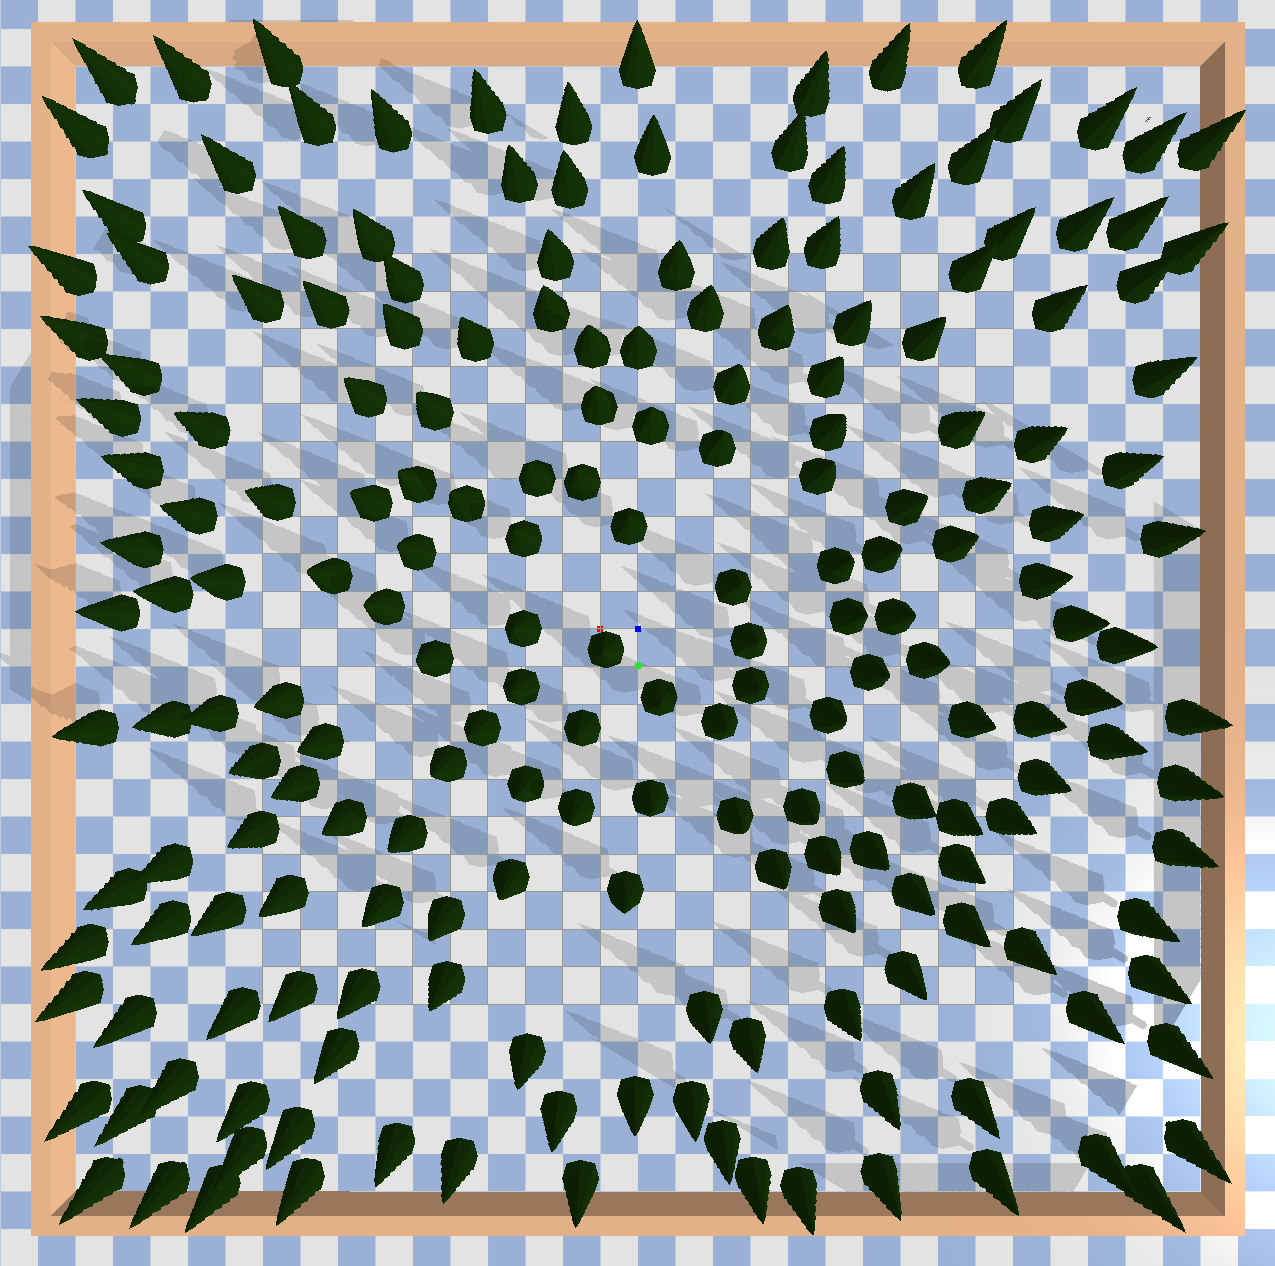
\includegraphics[scale=0.19]{images/SimulationImage.png}
\caption{Simulation (top view)}
\end{figure}


The simulation uses pybullet for physics and few control methods adapted from gym-pybullet-drones. Important parameters used for experimenting are - number of drones, number of trees and area size. For the most part we've used $3$ drones for exploring a forest area of $900m^2$ with $200$ trees (obstacles) as shown in Fig. 1. \\

\begin{figure}[h]
\centering
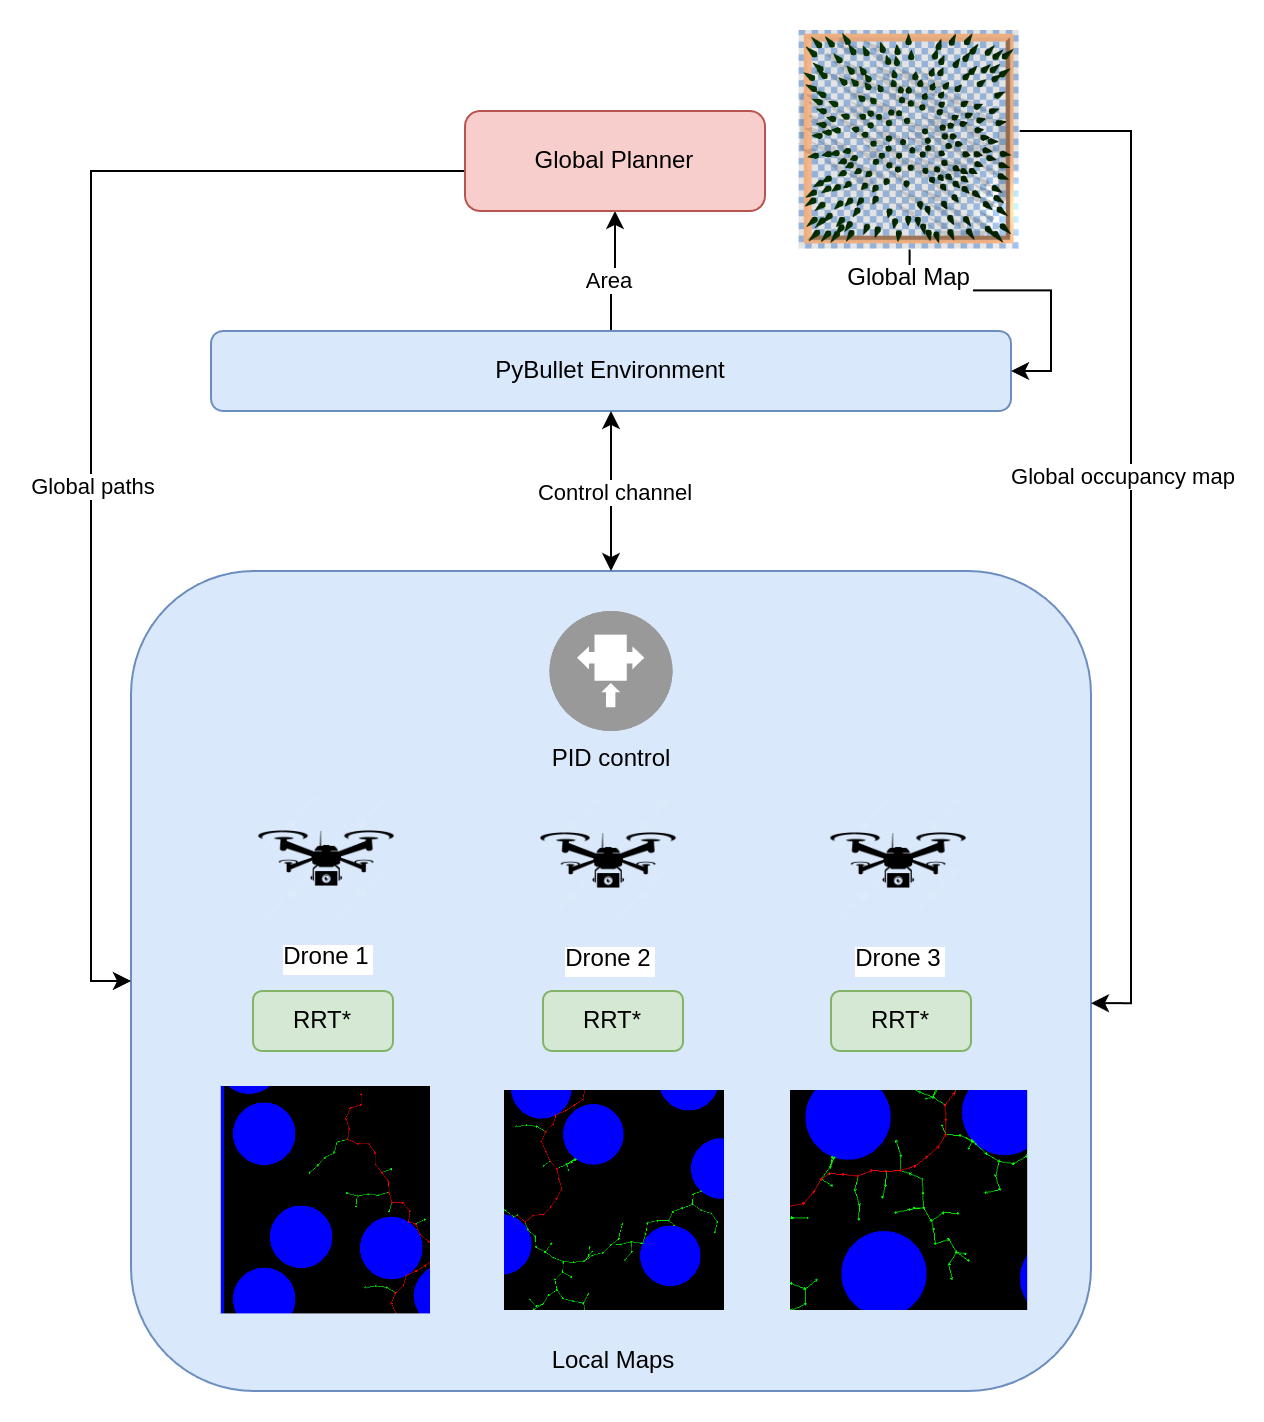
\includegraphics[scale=0.15]{images/arch_diag.png}
\caption{Architecture diagram}
\end{figure}

Other parameters include simulation frequency set at 48Hz. In each step/loop the next action is either executed or sampled (planned) for a drone.

Fig 2. represents a high level overview of how all processes tie in together to calculate and execute a obstacle free path.

\subsection{Results}
\begin{figure}[h]
\centering
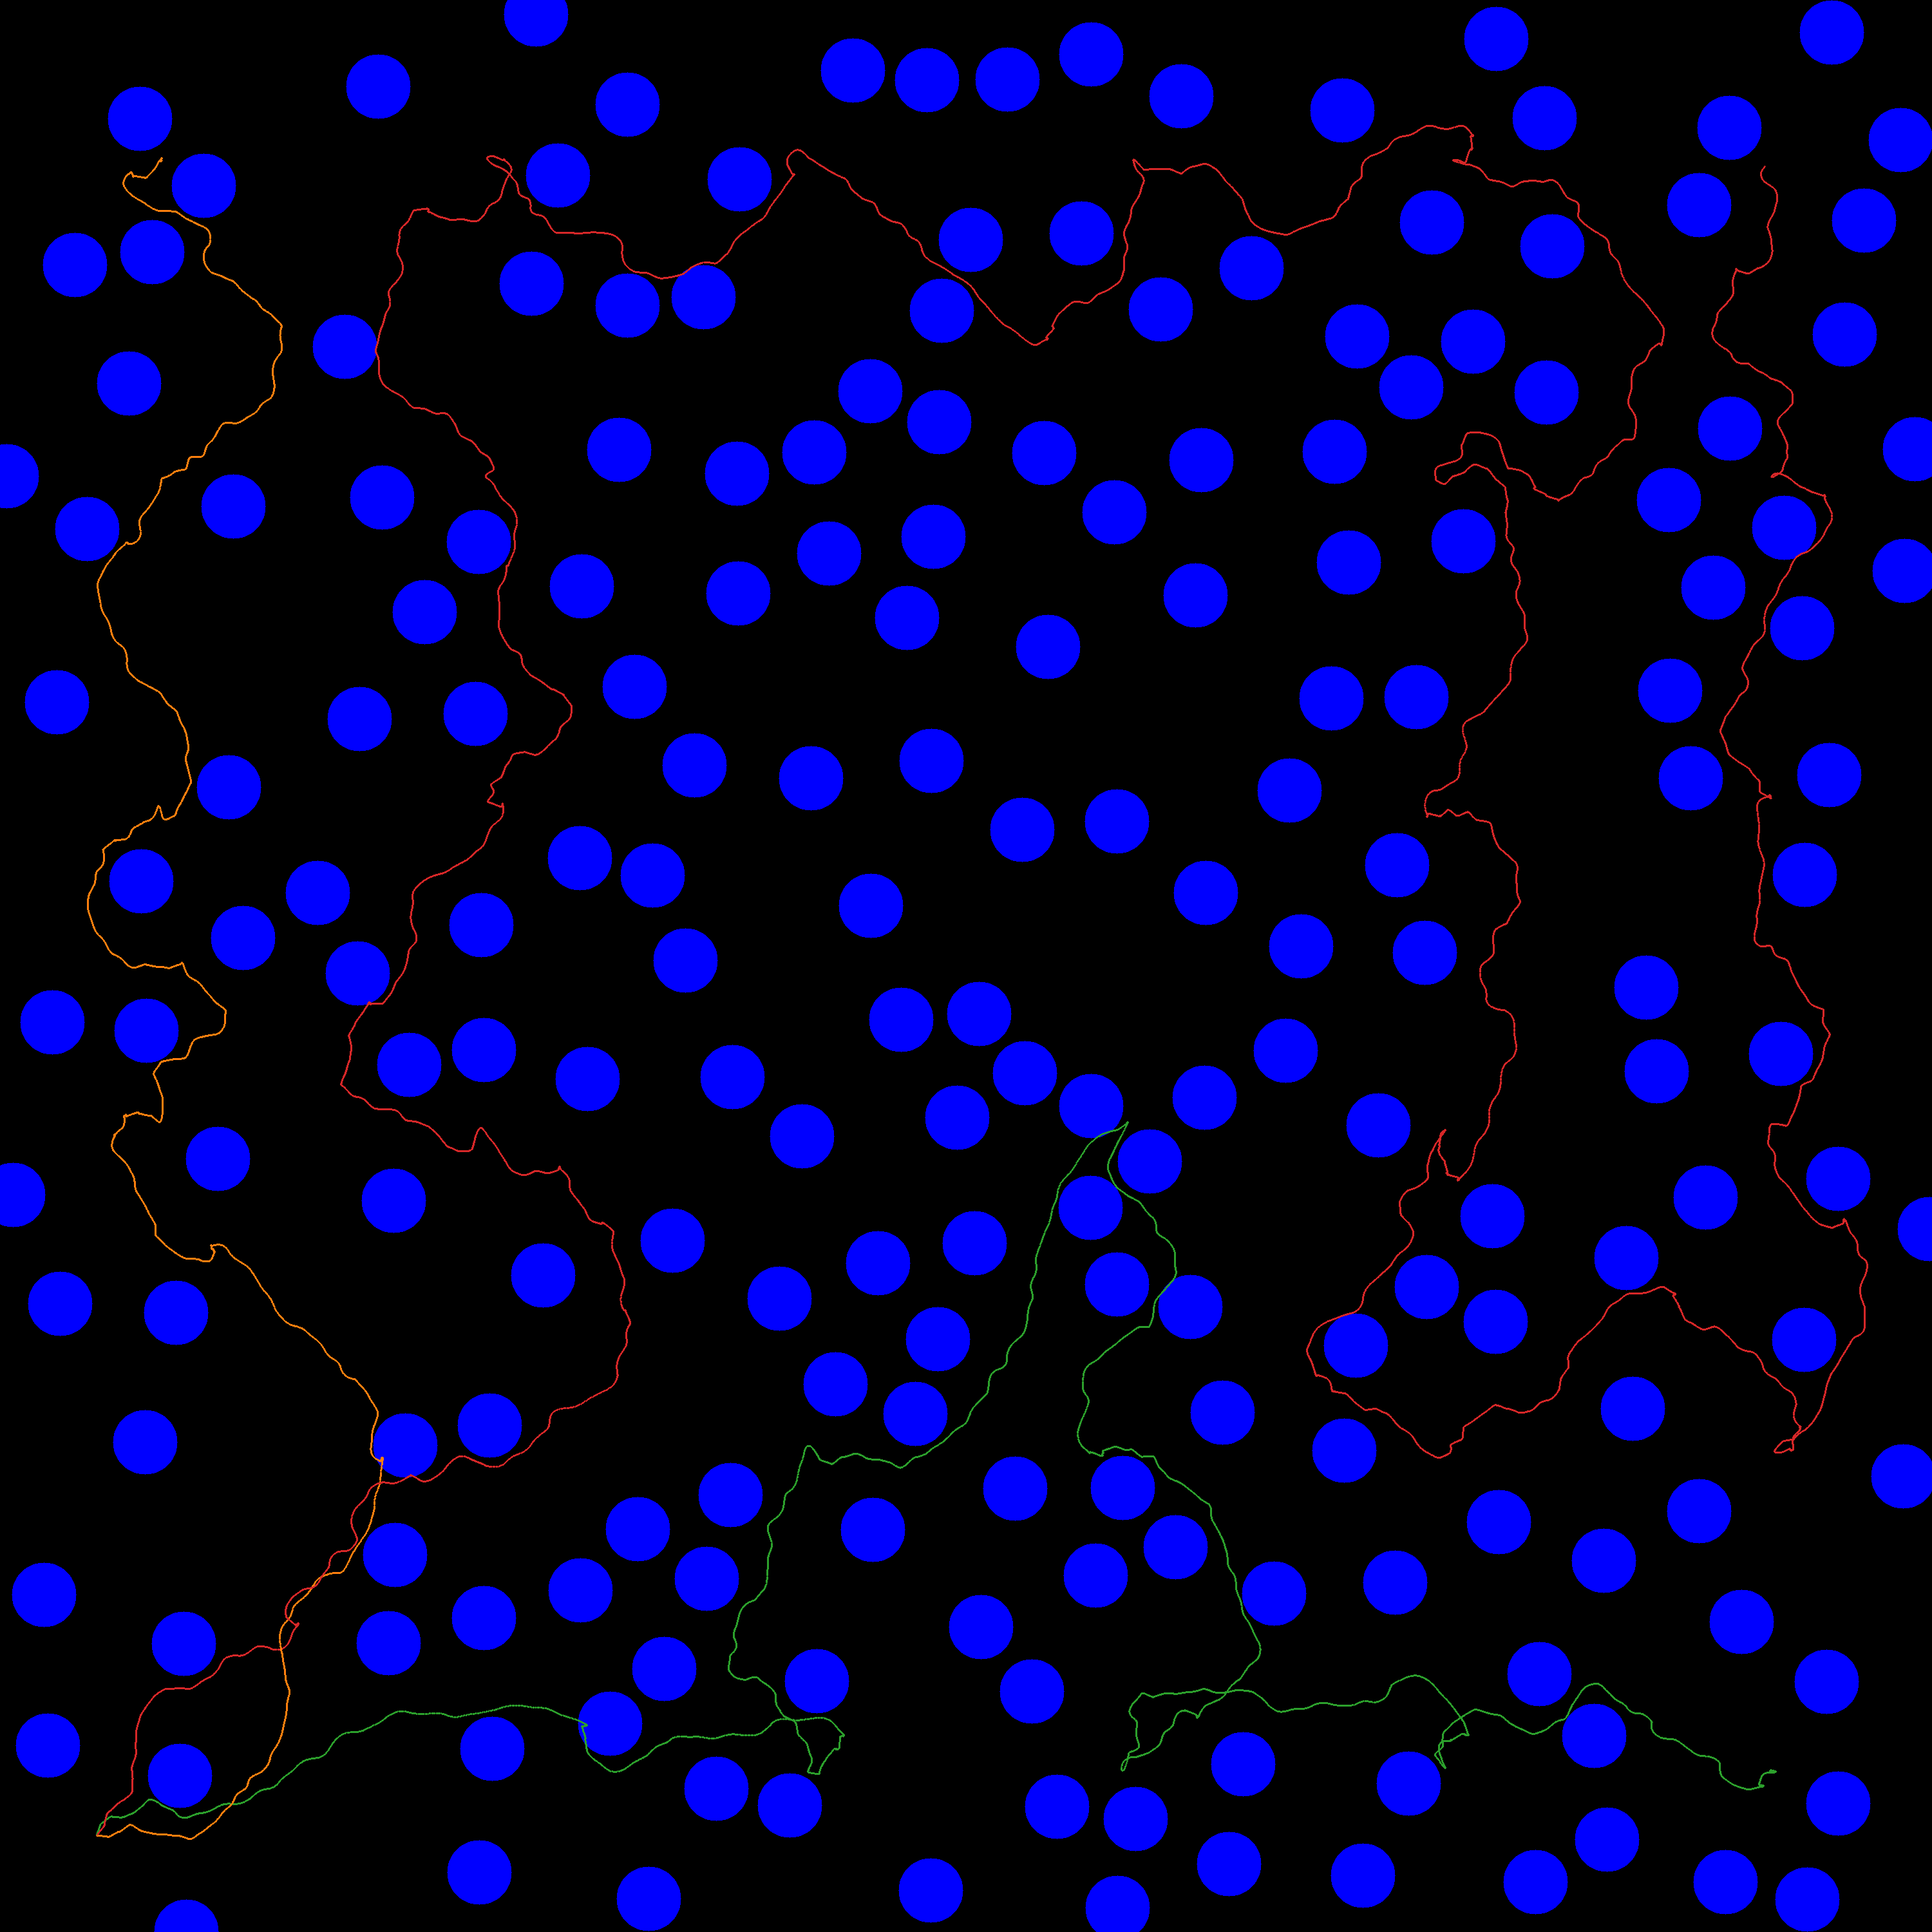
\includegraphics[scale=0.07]{images/preview_map_frame_11193.png}
\caption{Occupancy map on a 30 x 30 m area}
\end{figure}

\begin{figure}[h]
\centering
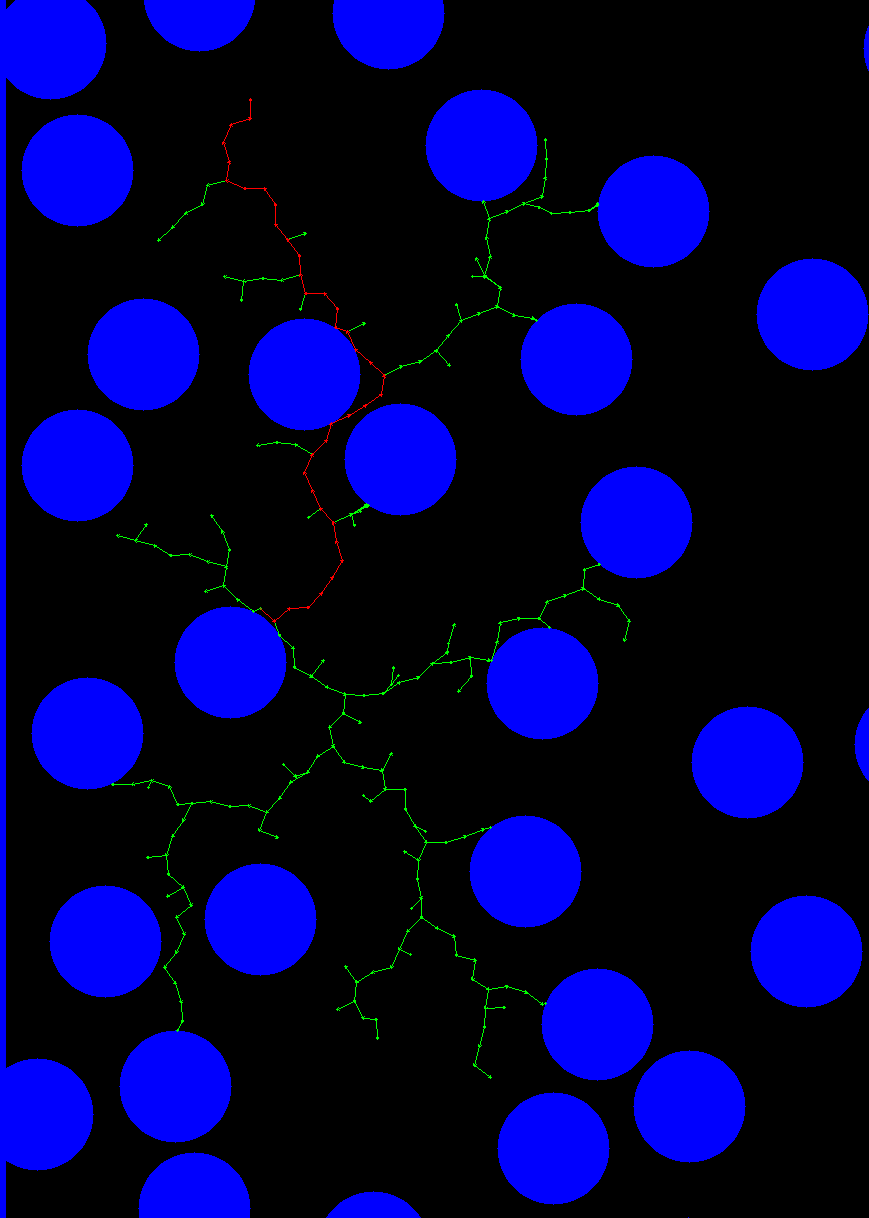
\includegraphics[scale=0.20]{images/rrt_drone_1_iter_6.png}
\caption{RRT on a local occupancy map}
\end{figure}

This \href{https://www.youtube.com/watch?v=JBWNEh0Fis4&ab_channel=ShantnavAgarwal}{video} shows drones navigating in the aforementioned setup.\\

Fig. 3 shows paths followed by each drone to explore the map using paths provided by global path planner and RRT algorithm, which took 8 hours in simulation time (3 mins in practice). \\

%[picture] shows the simulation running in a smaller area of $400m^2$ with $100$ trees took x mins. \\

Fig. 4 shows the RRT trees in a local map. As shown the drone doesn't have to know its final goal postion and such a series of local maps can guide the drone towards the goal while offering benefits of faster computation.
\section{DISCUSSION}
\subsection{Path planning and Control}

\begin{figure}[h]
\centering
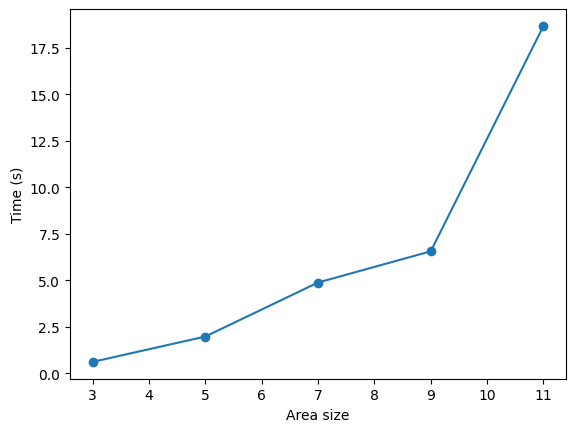
\includegraphics[scale=0.5]{images/time_area.png}
\caption{Area to explore vs time for finding path}
\end{figure}


As shown in Figure 3, the computation time tends to increase exponentially with area, and so we've solved RRTs on smaller areas.
The total time combined for solving RRTs on smaller maps is lesser than finding a path on the entire area.

RRTs produce a collision-free path, but they are neither smooth nor optimal.
A smooth path that adheres to the differential flatness property of a drone (i.e., four times differentiable) will allow us to directly calculate the required rotor torques for controlling the drone.
Using this information, a better controller with feed-forward control can be implemented.
Webb et al. introduced a Kindodynamic $RRT^*$ algorithm that exactly and optimally connects any pair of states for any system with controllable linear dynamics in state spaces of arbitrary dimensions\cite{DBLP:journals/corr/abs-1205-5088}.
With this improvement, the drone can fly faster and cover more distance as well.
In terms of improvements, the differential flatness property of a drone can be exploited to control motion upto the fourth derivative and generate smoother paths and simplifying trajectory generation.

 
\subsection{Global planner}

The global planner provides a series of goals for every drone in the global frame, scouting the entire region. This is done by converting the grid into cells and providing separate paths for each drone to visit. This is indeed practical and efficient as it provides continuous cell path by covering immediate neighbouring cells.

In practice, the global planner could use a satellite image of a forest and plan drones to cover it. 


\subsection{Local maps}

To reduce overall computation time, RRT computes multiple obstacle free paths
using a series of local maps to reach the global goal. This is done by slicing sections of the global occupancy map just enough to include the next goal given by the global planner to avoid use of a global occupancy map. The area vs time figure clearly shows that local maps of small areas combined would take shorter time to compute compared to the exponential increase of using a single global map.

\subsection{Obstacle detections}
With that said, all obstacles are revealed within a local map for the drone to compute a obstacle free path. The local map's dimensions can differ depending on the global map and grid size, which means detecting all obstacles within a local map is unlikely in the real world where sensors have a limited range of detection. \\
 A potential improvement here to imitate a real world scenario is using a dynamic local map and revealing obstacles only within a certain radius of the drone.

  
 

\addtolength{\textheight}{-12cm}  % This command serves to balance the column lengths
                                  % on the last page of the document manually. It shortens
                                  % the textheight of the last page by a suitable amount.
                                  % This command does not take effect until the next page
                                  % so it should come on the page before the last. Make
                                  % sure that you do not shorten the textheight too much.

%%%%%%%%%%%%%%%%%%%%%%%%%%%%%%%%%%%%%%%%%%%%%%%%%%%%%%%%%%%%%%%%%%%%%%%%%%%%%%%%



%%%%%%%%%%%%%%%%%%%%%%%%%%%%%%%%%%%%%%%%%%%%%%%%%%%%%%%%%%%%%%%%%%%%%%%%%%%%%%%%



%%%%%%%%%%%%%%%%%%%%%%%%%%%%%%%%%%%%%%%%%%%%%%%%%%%%%%%%%%%%%%%%%%%%%%%%%%%%%%%%



\printbibliography

\end{document}